% Provenance (never printed): old premiere S material on the history of plate
% tectonics (from continental drift to seafloor spreading: the ridges, the
% magnetic stripes, the ages of the drilled floor); see
% sources/book2/PROVENANCE.md. Profiles are computed in
% figdata/grade-11/magnetic_stripes.py, the age map in seafloor_age.py, the
% drilling fit in sediment_ages.py.
\chapter{Van continentverschuiving tot oceaanbodemspreiding}\label{ch:g11:drift-to-spreading}

Begin jaren 1950 zat in het Lamont-laboratorium van Columbia University een jonge
geologe, Marie Tharp, voor lange rijen getallen. Elk getal was een diepte van de
noordelijke Atlantische Oceaan, gemeten door het echolood van een schip, de ene
na de andere langs de koers van het schip. Door ze een voor een uit te zetten,
tekende ze de vorm van de oceaanbodem langs de koersen van schepen die de oceaan
waren overgestoken. Midden in de oceaan rees de bodem op tot een bergketen --- en
op elke koers zakte de bodem langs de kam van de keten weer weg in een diepe
kloof, alsof de bergen in het midden waren gespleten. Dit hoofdstuk volgt hoe
zulke metingen van de oceaanbodem een verworpen idee, de verschuiving van de
continenten, tot een theorie maakten: de oceaanbodem wordt bij de ruggen gemaakt
en schuift er vanaf, en hij draagt in zijn gesteenten een verslag van zijn eigen
ouderdom.
% ledger: aip:tharp, aip:featureless, usgs:echo-sounding

\begin{recall}
Continentverschuiving is het idee dat de continenten bewegen; Alfred Wegener
verdedigde het vanaf 1912 met de passende kustlijnen, fossielen, gesteenten en
oude klimaten, maar kon niet zeggen wat ze bewoog. Het aardoppervlak bestaat uit
starre platen, die elkaar ontmoeten bij divergente, convergente en transforme
grenzen; ze bewegen een paar centimeter per jaar, en $\qty{1}{cm}$ per jaar is
$\qty{10}{km}$ per miljoen jaar (Boek 1, jaar 7). De oceaanbodem heeft zijn
continentaal plat, zijn abyssale vlakten, zijn ruggen en zijn troggen (Boek 1,
jaar 8). De Aarde heeft een magnetisch veld, met een magnetische noord- en
zuidpool, dat een kompasnaald volgt; een geluidspuls die in het water wordt
gestuurd, keert terug als echo na een tijd die de afstand geeft (de
natuurkundeboeken).
\end{recall}

\section{Waarom continentverschuiving werd verworpen}

Wegeners bewijzen toonden dat de continenten ooit aan elkaar vastzaten. Wat ze
niet toonden, was hoe ze konden zijn verschoven. Wegener stelde zich voor dat de
continenten zich door het gesteente van de oceaanbodem ploegden, en natuurkundigen
antwoordden dat geen enkele bekende kracht een continent door vast gesteente kon
duwen zonder het te verbrijzelen. Een halve eeuw lang concludeerden de meeste
geologen dat de continenten helemaal niet waren verschoven.
% ledger: usgs:wegener-1912, usgs:jeffreys (Book 1 rows)

Er ontbraken twee dingen. Het eerste was een mechanisme. Het tweede, dat tot het
eerste leidde, was kennis van de bodem van de oceanen, die het grootste deel van
het aardoppervlak bedekt en die in 1912 vrijwel niemand had gezien: men nam aan
dat het een bijna vormloze vlakte was.
% ledger: aip:tharp, aip:featureless

\section{De oceaanbodem in kaart brengen}

Een echolood stuurt een korte geluidspuls van de romp van een schip naar de
zeebodem en meet de tijd tot de echo. Geluid plant zich in zeewater voort met
ongeveer \qty{1500}{m/s}; de puls gaat heen en terug, dus een vertraging $t$
betekent een diepte
\[
  d = \frac{v\,t}{2}.
\]
Een vertraging van \qty{6.0}{s} betekent bijvoorbeeld $1500 \times 6.0/2 =
\qty{4500}{m}$ water. In de negentiende eeuw werden diepten een voor een gemeten,
door een verzwaarde lijn naar de bodem te laten zakken. Na de Eerste
Wereldoorlog namen echoloden het over, en de registraties van hun echo's toonden
een bodem die veel ruiger was dan iemand had gedacht; in de jaren 1950 toonden
metingen van schepen van veel landen aan dat een grote bergketen op de oceaanbodem
bijna helemaal rond de Aarde loopt.
% ledger: noaa:sound-seawater, usgs:echo-sounding, usgs:line-soundings

\begin{history}[Marie Tharp en het riftdal, 1952]
% ledger: aip:tharp, aip:featureless
Vanaf 1947 had de geofysicus Bruce Heezen echolood-profielen verzameld over de
noordelijke Atlantische Oceaan. Marie Tharp, die toen niet aan boord van de
onderzoeksschepen mocht, maakte van wat ze later ``eindeloze rijen
dieptegetallen'' noemde tekeningen van de zeebodem. Tegen 1952, met de
oost-westkoersen van noord naar zuid op volgorde gelegd, zag ze dat één kenmerk
van koers tot koers op één lijn lag: een kloof langs de kam van de Midden-Atlantische
Rug, een riftdal. Heezen dacht eerst dat het een vergissing was. Toen bleken de
epicentra van de aardbevingen van de Atlantische Oceaan, op dezelfde schaal
uitgezet, in het riftdal zelf te liggen. De kaart van de oceaanbodem van de
wereld van Tharp en Heezen, in 1977 geschilderd door de kunstenaar Heinrich
Berann, gaf mensen het eerste realistische beeld van de oceaanbodem; in 1997
noemde de Library of Congress haar een van de vier grote cartografen van de
twintigste eeuw.
\end{history}

De mid-oceanische ruggen vormen één bijna doorlopend systeem van ongeveer
\qty{65000}{km} lang, voor meer dan negen tiende onder water; de kam ligt
gemiddeld \qty{2500}{m} onder het oppervlak. Langs de trage Midden-Atlantische Rug
wordt de kam doorsneden door een riftdal; langs de snellere Oost-Pacifische Rug is
hij een gladde, zacht glooiende top. De aardbevingen van de oceanen volgen de
ruggen op de voet. Alles wees erop dat er bij de rug iets
gebeurde --- maar wat?
% ledger: noaa:ridge, aip:tharp

\section{Oceaanbodemspreiding}

\begin{history}[Hess en de lopende band, 1962]
% ledger: usgs:hess, hess:1962
In 1962 publiceerde Harry Hess, geoloog aan Princeton University en admiraal bij
de marinereserve, \emph{History of Ocean Basins}.
Hij stelde voor dat heet gesteente onder de ruggen opstijgt en nieuwe oceaanbodem
wordt, die zich dan als een lopende band naar beide kanten verwijdert en bij de
troggen weer in de mantel wegzinkt. Robert Dietz, die op hetzelfde idee kwam, gaf
het zijn naam: \omterm{def:g11:drift-to-spreading:spreading}{oceaanbodemspreiding}. Het idee verklaarde waarom de Aarde niet
groeit, hoewel er voortdurend nieuwe bodem wordt gemaakt, waarom er zo weinig
sediment op de oceaanbodem ligt, en waarom de gesteenten van de oceaanbodem veel
jonger zijn dan die van de continenten.
\end{history}

\begin{definition}[Oceaanbodemspreiding]\label{def:g11:drift-to-spreading:spreading}
\emph{Oceaanbodemspreiding}\index{oceaanbodemspreiding} is het proces waarbij
langs de kam van een mid-oceanische rug nieuwe oceaanbodem ontstaat, waar
gesmolten gesteente uit de mantel opstijgt en stolt, en zich daarna naar beide
kanten van de rug verwijdert, zodat de oceaanbodem ouder wordt met de afstand tot
de rug.
\end{definition}

\begin{definition}[Spreidingssnelheid]\label{def:g11:drift-to-spreading:spreading-rate}
De \emph{volledige spreidingssnelheid}\index{spreidingssnelheid} van een rug is
de snelheid waarmee de twee platen aan weerszijden ervan uit elkaar gaan. De
\emph{halve spreidingssnelheid} is de snelheid waarmee de bodem aan één kant zich
van de as van de rug verwijdert. Bij symmetrische spreiding is de volledige
snelheid twee keer de halve.
\end{definition}

Ruggen spreiden met heel verschillende snelheden. De Midden-Atlantische Rug gaat
open met \qtyrange{2}{5}{cm} per jaar, de Oost-Pacifische Rug met
\qtyrange{6}{16}{cm} per jaar. Van de oceaanbodem die vandaag bestaat, werd
ongeveer een derde gemaakt bij trage ruggen (volledige snelheden van
\qtyrange{20}{55}{mm} per jaar) en ongeveer twee vijfde bij snelle
(\qtyrange{75}{180}{mm} per jaar).
% ledger: noaa:ridge, seton:rate-classes

Het idee van Hess was gedurfd, en aanvankelijk was er weinig rechtstreeks bewijs
voor. Het bewijs kwam uit twee onverwachte richtingen: het magnetisme van de
oceaanbodem en zijn sedimenten.

\section{Magnetische ompolingen en de gestreepte zeebodem}

\subsection{Een gesteente onthoudt het veld}

Het basalt van de oceaanbodem bevat kleine korrels magnetiet, een ijzeroxide dat
sterk magnetisch is. Wanneer basaltlava uitvloeit, is ze veel te heet om een
blijvende magnetisatie vast te houden; terwijl ze afkoelt, worden de korrels
gemagnetiseerd evenwijdig aan het aardmagnetisch veld om hen heen, en die richting
ligt daarna vast in het gesteente.
% ledger: usgs:magnetometers

\begin{definition}[Remanente magnetisatie; Curietemperatuur]\label{def:g11:drift-to-spreading:remanence}
De \emph{Curietemperatuur}\index{Curietemperatuur} van een magnetisch mineraal is
de temperatuur waarboven het geen eigen magnetisatie kan behouden: ongeveer
\qty{580}{\celsius} voor magnetiet. Een gesteente waarvan de magnetische korrels
in het aardmagnetisch veld onder hun Curietemperatuur afkoelen, behoudt een
magnetisatie evenwijdig aan het veld van dat moment, de
\emph{remanente magnetisatie}\index{remanente magnetisatie}. Ze blijft bestaan
lang nadat het veld is veranderd, tenzij het gesteente opnieuw boven de
Curietemperatuur wordt verhit.
\end{definition}
% ledger: tarduno:curie

\begin{omfigure}
\begin{tikzpicture}[font=\footnotesize, >={Stealth[length=5pt]}]
  % ground and lava flow
  \fill[lith basalt] (0,0) rectangle (11,0.6);
  \fill[omLithBasalt!45!red!35] (0,0.6) -- (11,0.6) -- (11,1.9) .. controls (9,2.0) and (4,2.15) .. (0,2.05) -- cycle;
  \fill[omLithBasalt!70] (0,1.35) -- (11,1.25) -- (11,1.9) .. controls (9,2.0) and (4,2.15) .. (0,2.05) -- cycle;
  \draw[black!60] (0,1.35) -- (11,1.25);
  \draw[line width=0.8pt] (0,2.05) .. controls (4,2.15) and (9,2.0) .. (11,1.9);
  \draw[black!60] (0,0.6) -- (11,0.6);
  % field lines (northern hemisphere: pointing down to the north)
  \foreach \x in {0.6,2.4,4.2,6.0,7.8,9.6} {
    \draw[->, omDef, line width=0.9pt] (\x,4.0) -- (\x+1.1,2.55);
  }
  \node[anchor=south west, text=omDef] at (0.2,4.05) {het magnetisch veld van de Aarde};
  % locked grains in the cooled top
  \foreach \x in {0.5,1.3,...,10.5} {
    \draw[->, black, line width=0.6pt] (\x,1.86) -- (\x+0.25,1.53);
  }
  % random grains in the hot interior
  \foreach \x/\a in {0.6/20,1.5/140,2.3/250,3.2/80,4.0/310,4.9/190,5.7/40,6.6/120,7.4/280,8.3/20,9.1/200,10.0/330} {
    \draw[->, black!55, line width=0.5pt] (\x,0.95) -- ++(\a:0.22);
  }
  \node[anchor=west, align=left] at (11.15,1.75) {afgekoeld onder \qty{580}{\celsius}: de\\korrels behouden de veldrichting};
  \node[anchor=west, align=left] at (11.15,0.92) {nog boven \qty{580}{\celsius}:\\geen blijvende magnetisatie};
  \node[anchor=west, align=left] at (11.15,0.25) {ouder gesteente};
  \node[anchor=west] at (9.0,4.25) {noord $\rightarrow$};
\end{tikzpicture}

{\small Een lavastroom die afkoelt (schematisch, noordelijk halfrond, waar het veld
naar het noorden en naar beneden wijst). De bovenkant van de stroom is afgekoeld
onder de \omterm{def:g11:drift-to-spreading:remanence}{Curietemperatuur} van magnetiet: de magnetische korrels (zwarte pijlen)
behouden de richting van het veld. Het binnenste, nog heter, legt nog niets vast;
het zal het veld vastleggen van het moment waarop het afkoelt.}
\end{omfigure}

\subsection{Het veld polt om}

Begin twintigste eeuw ontdekten Bernard Brunhes (in 1906) en daarna Motonori
Matuyama (in de jaren 1920) dat vulkanische gesteenten in twee groepen uiteenvallen.
In sommige wijst de magnetisatie dezelfde kant op als het huidige veld; in de
andere wijst ze de andere kant op, alsof de magnetische noord- en zuidpool van
plaats waren gewisseld. Het veld zelf was omgepoold, keer op keer.
% ledger: usgs:reversals

\begin{definition}[Magnetische ompoling; normale en omgekeerde polariteit]\label{def:g11:drift-to-spreading:reversal}
Een \emph{magnetische ompoling}\index{magnetische ompoling} is een verwisseling van
de magnetische noord- en zuidpool van de Aarde. Een tijd waarin het veld wees
zoals vandaag, is een tijd van \emph{normale polariteit}\index{normale polariteit};
een tijd waarin het de andere kant op wees, een tijd van \emph{omgekeerde
polariteit}\index{omgekeerde polariteit}. Een gesteente dat in een van beide
tijden is gemagnetiseerd, heeft dezelfde polariteit.
\end{definition}

Gedateerde lava's geven de opeenvolging van normale en omgekeerde intervallen: de
\emph{geomagnetische polariteitstijdschaal}. Haar lange intervallen zijn genoemd
naar wetenschappers die het magnetisme van de Aarde bestudeerden (Brunhes,
Matuyama, Gauss, Gilbert); de korte gebeurtenissen daarbinnen naar de plaatsen
waar ze het eerst werden gevonden.

\begin{omfigure}
\begin{tikzpicture}
\begin{axis}[width=0.92\linewidth, height=3.2cm, xmin=0, xmax=5.5, ymin=-0.9, ymax=1.9,
  axis y line=none, axis x line*=bottom, xtick={0,0.5,...,5.5}, tick label style={font=\small},
  xlabel={ouderdom (miljoen jaar)}, label style={font=\small}, clip=false]
\addplot[fill=black, draw=none] table {figdata/out/grade-11-magnetic_stripes-timescale.dat};
\draw[black] (axis cs:0,0) rectangle (axis cs:5.5,1);
\begin{scope}[every node/.style={font=\scriptsize, anchor=south}]
  \node at (axis cs:0.39,1.05) {Brunhes};
  \node at (axis cs:1.68,1.05) {Matuyama};
  \node at (axis cs:3.08,1.05) {Gauss};
  \node at (axis cs:4.74,1.05) {Gilbert};
\end{scope}
\draw[black!60] (axis cs:0.78,1) -- (axis cs:0.78,1.45);
\draw[black!60] (axis cs:2.581,1) -- (axis cs:2.581,1.45);
\draw[black!60] (axis cs:3.58,1) -- (axis cs:3.58,1.45);
\begin{scope}[every node/.style={font=\scriptsize, anchor=north}]
  \node at (axis cs:1.03,-0.05) {Jaramillo};
  \node at (axis cs:1.86,-0.05) {Olduvai};
\end{scope}
\node[font=\scriptsize, anchor=west] at (axis cs:5.55,0.75) {normaal};
\node[font=\scriptsize, anchor=west] at (axis cs:5.55,0.25) {(zwart)};
\end{axis}
\end{tikzpicture}

{\small De geomagnetische polariteitstijdschaal voor de laatste 5.5 miljoen jaar:
zwart voor \omterm{def:g11:drift-to-spreading:reversal}{normale polariteit}, wit voor omgekeerde. Het huidige normale interval
begon \num{780000} jaar geleden; er waren twintig ompolingen in de laatste vijf
miljoen jaar. Gegevens: Cande en Kent (1995).}
\end{omfigure}
% ledger: ck95:chrons

\subsection{Strepen op de oceaanbodem}

Vanaf de jaren 1950 sleepten schepen magnetometers achter zich aan over de oceanen,
en vonden dat het veld aan het zeeoppervlak niet het gladde veld was dat je van de
kern van de Aarde zou verwachten: het was hier iets sterker, daar iets zwakker.
% ledger: usgs:magnetometers

\begin{definition}[Magnetische anomalie]\label{def:g11:drift-to-spreading:anomaly}
Op een punt van het zeeoppervlak is de
\emph{magnetische anomalie}\index{magnetische anomalie} de gemeten sterkte van het
magnetisch veld min de sterkte die daar alleen op grond van het veld van de Aarde
wordt verwacht. Ze is positief waar de gesteenten eronder het veld versterken,
negatief waar ze ertegenin werken. Ze is klein vergeleken met het veld zelf, en
wordt gemeten in nanotesla (\unit{nT}).
\end{definition}

Over een groot gebied in kaart gebracht, tekenden de anomalieën strepen evenwijdig
aan de kam van de rug, afwisselend positief en negatief, als de vacht van een zebra
--- en het patroon aan de ene kant van de rug was het spiegelbeeld van het
patroon aan de andere kant.
% ledger: usgs:magnetometers

\begin{history}[Vine en Matthews, 1963]
% ledger: vm:1963, usgs:magnetometers
In september 1963 publiceerden Fred Vine en Drummond Matthews een kort artikel in het tijdschrift \emph{Nature},
\emph{Magnetic anomalies over oceanic ridges}. Ze brachten de spreiding van Hess
en de ompolingen van het veld samen. Als nieuwe bodem bij de kam ontstaat en
wegschuift terwijl het veld ompoolt, legt elke strook bodem de polariteit vast van
de tijd waarin ze afkoelde. De bodem wordt een gestreepte band die aan beide
kanten van de rug afrolt: positieve anomalieën boven normale stroken, negatieve
boven omgekeerde, dezelfde reeks aan beide kanten.
\end{history}

\begin{omfigure}
\begin{tikzpicture}
\begin{axis}[hide axis, axis equal image, width=0.94\linewidth, xmin=-320, xmax=420, ymin=-120, ymax=160, clip=false]
  % block faces
  \fill[white] (axis cs:-300,0) -- (axis cs:300,0) -- (axis cs:390,70) -- (axis cs:-210,70) -- cycle;
  \fill[omLithBasalt!25] (axis cs:-300,0) rectangle (axis cs:300,-60);
  \fill[omLithBasalt!45] (axis cs:300,0) -- (axis cs:390,70) -- (axis cs:390,10) -- (axis cs:300,-60) -- cycle;
  \addplot[fill=black!80, draw=none] table {figdata/out/grade-11-magnetic_stripes-block.dat};
  \draw[black] (axis cs:-300,0) -- (axis cs:300,0) -- (axis cs:390,70) -- (axis cs:-210,70) -- cycle;
  \draw[black] (axis cs:-300,0) -- (axis cs:-300,-60) -- (axis cs:300,-60) -- (axis cs:300,0);
  \draw[black] (axis cs:300,-60) -- (axis cs:390,10) -- (axis cs:390,70);
  % ridge axis
  \draw[omRidge, line width=1.6pt] (axis cs:0,0) -- (axis cs:90,70);
  \node[font=\footnotesize, text=omRidge, anchor=south] at (axis cs:90,72) {as van de rug};
  % rising magma
  \fill[red!60!orange, opacity=0.75] (axis cs:-12,-60) -- (axis cs:12,-60) -- (axis cs:3,0) -- (axis cs:-3,0) -- cycle;
  \draw[->, >={Stealth[length=5pt]}, red!70!black, line width=1pt] (axis cs:0,-95) -- (axis cs:0,-62);
  \node[font=\footnotesize, anchor=north] at (axis cs:0,-96) {gesmolten gesteente stijgt op};
  % spreading arrows
  \draw[->, >={Stealth[length=6pt]}, line width=1.2pt] (axis cs:-90,100) -- (axis cs:-220,100);
  \draw[->, >={Stealth[length=6pt]}, line width=1.2pt] (axis cs:150,100) -- (axis cs:280,100);
  \node[font=\footnotesize, anchor=south] at (axis cs:-155,103) {ouder};
  \node[font=\footnotesize, anchor=south] at (axis cs:215,103) {ouder};
  % legend
  \fill[black!80] (axis cs:-300,-100) rectangle (axis cs:-280,-88);
  \node[font=\footnotesize, anchor=west] at (axis cs:-276,-94) {normale polariteit};
  \draw[black] (axis cs:-300,-118) rectangle (axis cs:-280,-106);
  \node[font=\footnotesize, anchor=west] at (axis cs:-276,-112) {omgekeerde polariteit};
\end{axis}
\end{tikzpicture}

{\small De gestreepte oceaanbodem (schematisch, berekend voor een rug die aan elke
kant met \qty{7.5}{cm} per jaar spreidt, over de laatste 4 miljoen jaar). Elke
strook bodem behield de polariteit van het veld op het moment dat ze bij de as
afkoelde; het patroon aan de ene kant is het spiegelbeeld van dat aan de andere.}
\end{omfigure}

\begin{proposition}[Afstand van een streep tot de as]\label{prop:g11:drift-to-spreading:stripe}
Als een rug symmetrisch spreidt met een constante halve snelheid $u$, dan ligt de
bodem die een tijd $t$ geleden bij de as ontstond nu op een afstand
\[
  x = u\,t
\]
aan weerszijden van de as. In het bijzonder ligt de grens tussen twee strepen die
een ompoling met ouderdom $t$ vastlegt, aan beide kanten op de afstand $u\,t$.
\end{proposition}

\begin{proof}
Een stuk bodem dat een tijd $t$ geleden bij de as ontstond, heeft zich sindsdien
met de snelheid $u$ van de as verwijderd, gedurende de tijd $t$: het heeft de
afstand $u\,t$ afgelegd. Een stuk dat op hetzelfde moment aan de andere kant van
de as ontstond, beweegt met dezelfde snelheid de andere kant op, en ligt op
dezelfde afstand. De bodem aan weerszijden van een ompolingsgrens ontstond vlak voor
en vlak na de ompoling, dus de grens ligt waar bodem met ouderdom $t$ ligt: op $u\,t$.
\end{proof}

De anomalieën kunnen uit de tijdschaal worden berekend. In de profielen hieronder
is de gemagnetiseerde laag een plaat gesteente van \qty{1}{km} dik waarvan de
bovenkant \qty{3}{km} onder het zeeoppervlak ligt, met de propositie verdeeld in
blokken met normale en \omterm{def:g11:drift-to-spreading:reversal}{omgekeerde polariteit}; het veld van elk blok aan het
zeeoppervlak wordt opgeteld. Boven een brede strook is de anomalie het sterkst
bij de randen, waar de polariteit verandert, en zwakker boven het midden; maar
haar teken volgt de polariteit van de strook eronder.

\begin{omfigure}
\begin{tikzpicture}
\begin{axis}[omrecord, name=fast, width=0.92\linewidth, height=5.0cm, xmin=-375, xmax=375, ymin=-820, ymax=560,
  ytick={-400,0,400}, xtick={-300,-200,...,300}, tick label style={font=\small}, label style={font=\small},
  ylabel={anomalie (\unit{nT})}, title={\small snelle rug: halve snelheid \qty{7.5}{cm} per jaar}, clip=false]
\addplot[fill=black, draw=none] table[y expr=\thisrow{y}*55-700] {figdata/out/grade-11-magnetic_stripes-fastblocks.dat};
\draw[black] (axis cs:-375,-755) rectangle (axis cs:375,-645);
\addplot[omDef, line width=0.9pt] table[x=x_km, y=anomaly_nT] {figdata/out/grade-11-magnetic_stripes-fast.dat};
\draw[black!40] (axis cs:-375,0) -- (axis cs:375,0);
\draw[black!50, densely dashed] (axis cs:268.5,-645) -- (axis cs:268.5,560);
\draw[black!50, densely dashed] (axis cs:-268.5,-645) -- (axis cs:-268.5,560);
\node[font=\scriptsize, anchor=south west, fill=white, inner sep=1pt] at (axis cs:270,-610) {3.58 miljoen jaar};
\end{axis}
\begin{axis}[omrecord, at={(fast.south)}, anchor=north, yshift=-1.6cm, width=0.92\linewidth, height=5.0cm,
  xmin=-62.5, xmax=62.5, ymin=-820, ymax=560, ytick={-400,0,400}, xtick={-60,-40,...,60},
  tick label style={font=\small}, label style={font=\small},
  ylabel={anomalie (\unit{nT})}, xlabel={afstand tot de as van de rug (\unit{km})},
  title={\small trage rug: halve snelheid \qty{1.25}{cm} per jaar}, clip=false]
\addplot[fill=black, draw=none] table[y expr=\thisrow{y}*55-700] {figdata/out/grade-11-magnetic_stripes-slowblocks.dat};
\draw[black] (axis cs:-62.5,-755) rectangle (axis cs:62.5,-645);
\addplot[omProp, line width=0.9pt] table[x=x_km, y=anomaly_nT] {figdata/out/grade-11-magnetic_stripes-slow.dat};
\draw[black!40] (axis cs:-62.5,0) -- (axis cs:62.5,0);
\draw[black!50, densely dashed] (axis cs:44.75,-645) -- (axis cs:44.75,560);
\draw[black!50, densely dashed] (axis cs:-44.75,-645) -- (axis cs:-44.75,560);
\node[font=\scriptsize, anchor=south west, fill=white, inner sep=1pt] at (axis cs:45,-610) {3.58 miljoen jaar};
\end{axis}
\end{tikzpicture}

{\small Magnetische anomalieën, uit de polariteitstijdschaal berekend over een
snelle en een trage rug, voor bodem tot 5 miljoen jaar oud aan elke kant. Onder
elk profiel de stroken bodem (zwart: normaal; wit: omgekeerd). De anomalie is
positief boven normale stroken en negatief boven omgekeerde; ze verandert van
teken bij de grenzen. De stippellijnen markeren de grens van 3.58 miljoen jaar.
Let op de verschillende afstandsschalen: de trage rug perst dezelfde geschiedenis
in een zesde van de breedte, en zijn kortste gebeurtenissen vloeien in elkaar
over. Een model berekend met gekozen waarden (een laag gemagnetiseerd met
\qty{5}{A/m}, verticaal gemagnetiseerd, zoals op hoge breedten); tijdschaal naar
Cande en Kent (1995).}
\end{omfigure}
% values computed in figdata/grade-11/magnetic_stripes.py; ledger: ck95:chrons

\begin{method}[Een spreidingssnelheid uit een magnetisch profiel]\label{met:g11:drift-to-spreading:rate}
\begin{enumerate}
  \item Zoek de as van de rug: het symmetriemiddelpunt van het profiel, in het
        midden van de centrale positieve anomalie.
  \item Herken aan beide kanten een ompolingsgrens --- een tekenwisseling van de
        anomalie die de tijdschaal dateert --- en meet aan elke kant haar afstand
        tot de as.
  \item Deel elke afstand door de ouderdom van de ompoling: dat geeft de halve
        snelheid aan elke kant, in kilometer per miljoen jaar
        ($\qty{10}{km}$ per miljoen jaar is $\qty{1}{cm}$ per jaar).
  \item Tel de twee halve snelheden op om de volledige snelheid te krijgen.
\end{enumerate}
\end{method}

\begin{example}[De snelle rug]\label{ex:g11:drift-to-spreading:fast}
Op het snelle profiel ligt de grens tussen de intervallen Gauss en Gilbert,
\num{3.58} miljoen jaar oud, aan elke kant \qty{268.5}{km} van de as.
De halve snelheid is $268.5/3.58 = \qty{75}{km}$ per miljoen jaar, dat is
\qty{7.5}{cm} per jaar; de volledige snelheid is \qty{15}{cm} per jaar, de
snelheid van de snelste delen van de Oost-Pacifische Rug.
\end{example}
% values computed in figdata/grade-11/magnetic_stripes.py (fast_gg_km 268.5)

De magnetische strepen doen meer dan de spreiding bevestigen: zodra een profiel
aan de tijdschaal is gekoppeld, geeft elke streep de ouderdom van de bodem
eronder. In de jaren 1960 werden oudere strepen gedateerd door een constante
snelheid aan te nemen; een toets van de hele theorie was de bodem op een totaal
andere manier te dateren.
% ledger: whoi:h68

\section{Ouderdom uit de sedimenten}

Sediment --- de schaaltjes van piepkleine plankton, klei, stof --- zakt langzaam
naar de oceaanbodem en hoopt zich erop op. Het oudste sediment dat direct op het
basalt ligt, werd kort na het ontstaan van het basalt afgezet; zijn fossielen, die
van tijdperk tot tijdperk veranderen, dateren het.

In 1968 stak het boorschip \emph{Glomar Challenger}, gebouwd om in de diepe
oceaanbodem te boren en boorkernen mee terug te brengen, de Midden-Atlantische Rug
over tussen Zuid-Amerika en Afrika. Op zeven plaatsen langs een lijn bij
breedte \ang{30} ZB boorde het door het sediment heen tot in het basalt eronder,
op afstanden van \qty{191}{km} tot \qty{1270}{km} van de as van de rug.
% ledger: usgs:glomar, dsdp3:rate, dsdp3:table5

\begin{omfigure}
\begin{tikzpicture}
\begin{axis}[omrecord, width=0.8\linewidth, height=6.2cm, xmin=0, xmax=1400, ymin=0, ymax=80,
  xlabel={afstand tot de as van de rug (\unit{km})}, ylabel={ouderdom (miljoen jaar)},
  tick label style={font=\small}, label style={font=\small}, legend pos=north west,
  legend style={font=\scriptsize, cells={anchor=west}}]
\addplot[omProp, line width=0.9pt, domain=0:1400] table[x=dist_km, y=age] {figdata/out/grade-11-sediment_ages-fit.dat};
\addplot[only marks, mark=*, mark size=2pt, omDef, error bars/.cd, x dir=both, x explicit, y dir=both, y explicit]
  table[x=dist_km, y=age, x error=dist_err, y error=age_err] {figdata/out/grade-11-sediment_ages-sites.dat};
\addplot[only marks, mark=square, mark size=2.2pt, black] table[x=dist_km, y=age] {figdata/out/grade-11-sediment_ages-magnetic.dat};
\legend{{constante halve snelheid \qty{1.9}{cm} per jaar}, {oudste sediment (fossielen)}, {magnetische strepen}}
\node[font=\scriptsize, anchor=north west] at (axis cs:195,9.5) {16};
\node[font=\scriptsize, anchor=north west] at (axis cs:384,22.5) {15};
\node[font=\scriptsize, anchor=south east] at (axis cs:502,27) {18};
\node[font=\scriptsize, anchor=north west] at (axis cs:647,31.5) {17};
\node[font=\scriptsize, anchor=south east] at (axis cs:723,41) {14};
\node[font=\scriptsize, anchor=north west] at (axis cs:994,47.5) {19};
\node[font=\scriptsize, anchor=south east] at (axis cs:1266,68) {20};
\end{axis}
\end{tikzpicture}

{\small Ouderdom van het oudste sediment op het basalt op de zeven boorplaatsen van
1968 (genummerd), tegen hun afstand tot de as van de Midden-Atlantische Rug; de
vierkantjes geven de ouderdom van de magnetische strepen op de plaatsen waar die
werden herkend. De lijn is de constante halve snelheid die het best bij de
ouderdommen van het sediment past. Gegevens: Deep Sea Drilling Project, Leg 3 (1970).}
\end{omfigure}
% ledger: dsdp3:table5 (fit computed in figdata/grade-11/sediment_ages.py)

De ouderdom neemt gestaag toe met de afstand tot de rug, aan beide kanten ervan:
de twee plaatsen die aan de Afrikaanse kant werden aangeboord, liggen op dezelfde
lijn als die aan de Amerikaanse kant. De best passende constante halve snelheid is
\qty{1.9}{cm} per jaar, en de ouderdommen uit de fossielen komen overeen met die
welke de magnetische strepen voorspellen. De wetenschappers van de expeditie
concludeerden dat de bodem minstens de laatste 66 miljoen jaar met iets minder
dan \qty{2}{cm} per jaar aan elke kant was gespreid. De \omterm{def:g11:drift-to-spreading:spreading}{oceaanbodemspreiding} had
een toets doorstaan waarvoor ze had kunnen zakken.
% ledger: dsdp3:rate, dsdp3:table5 (rate_palaeo_cm_yr 1.90 in figdata/grade-11/sediment_ages.py)

\begin{omfigure}
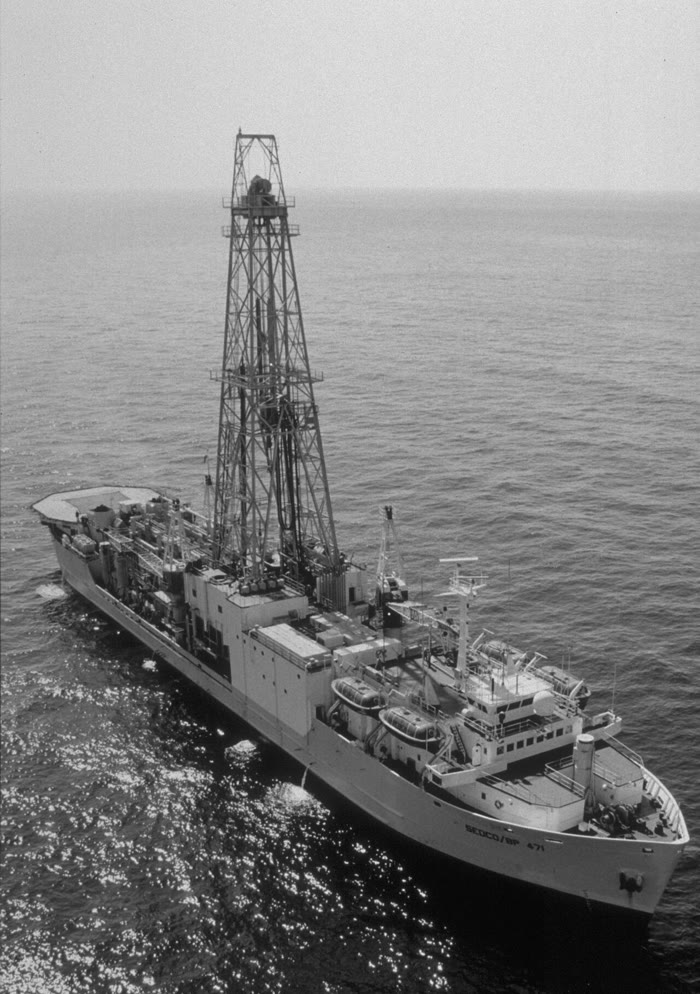
\includegraphics[width=0.36\linewidth]{images/book2/g11-odp-joides-resolution.jpg}

{\small Het boorschip \emph{JOIDES Resolution}, de opvolger van de
\emph{Glomar Challenger}: de hoge toren is de boortoren, en het schip
vervoert meer dan \qty{9000}{m} boorbuis. Foto: Ocean Drilling Program, Texas A\&M
University (publiek domein).}
\end{omfigure}
% ledger: photo:g11-joides, usgs:glomar

Sindsdien zijn duizenden magnetische profielen en honderden boorgaten samengevoegd
tot een kaart van de ouderdom van de hele oceaanbodem.

\begin{omfigure}
\begin{tikzpicture}
\begin{axis}[ommap, width=\linewidth, xtick=\empty, ytick=\empty, grid=none,
    axis background/.style={}, clip=true, name=map]
  \addplot graphics[xmin=-180, xmax=180, ymin=-90, ymax=90] {figdata/out/grade-11-seafloor_age.png};
  \addplot[black!60, line width=0.15pt] table {figdata/out/shared-geo-land.dat};
\end{axis}
\begin{axis}[at={(map.south)}, anchor=north, yshift=-0.35cm, scale only axis, width=0.55\linewidth, height=0.32cm,
    xmin=0, xmax=200, ymin=0, ymax=1, axis y line=none, axis x line*=bottom,
    xtick={0,20,...,180}, tick label style={font=\scriptsize},
    xlabel={ouderdom van de oceaanbodem (miljoen jaar); grijs: geen oceaanbodem}, label style={font=\scriptsize},
    enlargelimits=false]
  \addplot graphics[xmin=0, xmax=200, ymin=0, ymax=1] {figdata/out/grade-11-seafloor_age-bar.png};
\end{axis}
\end{tikzpicture}

{\small De ouderdom van de oceaanbodem. Het jongst (rood) langs de ruggen, wordt
hij aan beide kanten ouder naarmate hij er verder vandaan ligt; de oudste bodem
(blauw en paars) ligt aan de randen van de oceanen, tegen de continenten en langs
de troggen. Gegevens: Seton en anderen (2020), in cellen van 1 graad; contouren
van het land: Natural Earth.}
\end{omfigure}
% ledger: data:b2-seafloor-age, data:ne-land (map computed in figdata/grade-11/seafloor_age.py)

De kaart bevestigt alles tegelijk. Langs elke rug is de bodem jong, en zijn
ouderdom neemt symmetrisch toe naarmate je je ervan verwijdert. Geen enkele
oceaanbodem is ouder dan ongeveer \num{190} miljoen jaar: de oudste ligt in het
westen van de Grote Oceaan en voor de oostkust van Noord-Amerika (een paar kleine
bekkens in het oosten van de Middellandse Zee worden apart geteld). De gemiddelde
ouderdom van de oceaanbodem is ongeveer \num{64} miljoen jaar, en ongeveer drie
kwart ervan is jonger dan 100 miljoen jaar --- terwijl de continenten veel oudere
gesteenten bewaren. De oceaanbodem is jong omdat hij voortdurend bij de ruggen
wordt gemaakt en, zoals Hess zag, ergens anders wordt vernietigd: waar, is het
onderwerp van \cref{ch:g11:subduction-zones}.
% ledger: data:b2-seafloor-age (oldest_open_myr 192.5, share_younger_100 0.76 in figdata/grade-11/seafloor_age.py), seton:mean-age, usgs:hess

\section{Oefeningen}

\begin{exercise}[$\star$]\label{exo:g11:drift-to-spreading:1}
Definieer \omterm{def:g11:drift-to-spreading:spreading}{oceaanbodemspreiding}. Wat is het verschil tussen de volledige en de
halve \omterm{def:g11:drift-to-spreading:spreading-rate}{spreidingssnelheid} van een rug?
\end{exercise}

\begin{exercise}[$\star$]\label{exo:g11:drift-to-spreading:2}
Waarom legt een lava de richting van het aardmagnetisch veld pas vast als ze is
afgekoeld onder ongeveer \qty{580}{\celsius}? Wat gebeurt er met dat verslag als
het gesteente later tot \qty{700}{\celsius} wordt verhit?
\end{exercise}

\begin{exercise}[$\star$]\label{exo:g11:drift-to-spreading:3}
Een echolood hoort de echo van zijn puls \qty{5.2}{s} nadat het hem uitzond.
Hoe diep ligt de zeebodem, als je voor de geluidssnelheid in zeewater
\qty{1500}{m/s} neemt?
\end{exercise}

\begin{exercise}[$\star$]\label{exo:g11:drift-to-spreading:4}
Op de polariteitstijdschaal van dit hoofdstuk: hoe lang duurt het huidige normale
interval al? Hoe lang duurde de Jaramillo-gebeurtenis? Hoeveel ompolingen vonden
er plaats in de laatste vijf miljoen jaar?
\end{exercise}

\begin{exercise}[$\star$]\label{exo:g11:drift-to-spreading:5}
De mid-oceanische ruggen zijn ongeveer \qty{65000}{km} lang. De omtrek van de
Aarde is ongeveer \qty{40000}{km}. Hoeveel keer zouden de ruggen rond de Aarde
gaan?
\end{exercise}

\begin{exercise}[$\star\star$]\label{exo:g11:drift-to-spreading:6}
Op een magnetisch profiel ligt de grens tussen de intervallen Brunhes en Matuyama
(\num{0.78} miljoen jaar) \qty{20}{km} van de as van de rug. Bereken de halve en
de volledige snelheid in centimeter per jaar.
\end{exercise}

\begin{exercise}[$\star\star$]\label{exo:g11:drift-to-spreading:7}
Op een ander profiel ligt de grens Gauss--Gilbert (\num{3.58} miljoen jaar)
\qty{45}{km} ten westen en \qty{44}{km} ten oosten van de as. Bereken de halve
snelheid aan elke kant en de volledige snelheid. Is de spreiding symmetrisch?
\end{exercise}

\begin{exercise}[$\star\star$]\label{exo:g11:drift-to-spreading:8}
Boorplaats 19 van 1968 ligt \qty{990}{km} van de as van de Midden-Atlantische
Rug. Voorspel met een halve snelheid van \qty{1.9}{cm} per jaar de ouderdom van
de bodem daar, en vergelijk met de \num{49} miljoen jaar van het oudste sediment
ervan.
\end{exercise}

\begin{exercise}[$\star\star$]\label{exo:g11:drift-to-spreading:9}
Een rug spreidt met een halve snelheid van \qty{2}{cm} per jaar. Geef met de
tijdschaal van dit hoofdstuk de afstanden tot de as van de grenzen bij 0.78,
0.99, 1.07, 1.77 en 1.95 miljoen jaar, en teken de strepen aan één kant, normaal
in het zwart.
\end{exercise}

\begin{exercise}[$\star\star$]\label{exo:g11:drift-to-spreading:10}
De gemiddelde ouderdom van de oceaanbodem is ongeveer \num{64} miljoen jaar; de
Aarde is ongeveer \num{4.6} miljard jaar oud. Welk deel van de ouderdom van de
Aarde is dat? Welk argument van Hess ondersteunt het?
\end{exercise}

\begin{exercise}[$\star\star$]\label{exo:g11:drift-to-spreading:11}
Leg met een tekening uit waarom het patroon van magnetische strepen aan de ene
kant van een rug het spiegelbeeld is van het patroon aan de andere kant. Wat zou
deze symmetrie verbreken?
\end{exercise}

\begin{exercise}[$\star\star\star$]\label{exo:g11:drift-to-spreading:12}
Stel dat de ruggen, in totaal \qty{65000}{km} lang, spreiden met een gemiddelde
volledige snelheid van \qty{5}{cm} per jaar.
\begin{enumerate}
  \item Welke oppervlakte nieuwe oceaanbodem maken ze elk jaar, in \unit{km^2}?
  \item De oceaanbodem beslaat ongeveer \qty{2.9e8}{km^2}. Hoe lang zouden de
        ruggen erover doen om zoveel te maken?
  \item Vergelijk met de oudste oceaanbodem, ongeveer \num{190} miljoen jaar.
        Wat moet er met de oceaanbodem gebeuren, even snel als hij wordt gemaakt?
\end{enumerate}
\end{exercise}

\begin{exercise}[$\star\star\star$]\label{exo:g11:drift-to-spreading:13}
De Jaramillo-gebeurtenis duurde van \num{0.99} tot \num{1.07} miljoen jaar geleden.
Hoe breed is haar streep aan elke kant van een rug met een halve snelheid van
\qty{1.25}{cm} per jaar, en van een rug met \qty{7.5}{cm} per jaar? Het
gemagnetiseerde gesteente ligt ongeveer \qty{3}{km} onder het zeeoppervlak. Leg
uit waarom de gebeurtenis duidelijk te zien is op het snelle profiel van dit
hoofdstuk, maar nauwelijks op het trage.
\end{exercise}

\begin{exercise}[$\star\star\star$]\label{exo:g11:drift-to-spreading:14}
Op de boorplaatsen van 1968 is het sediment \qty{176}{m} dik op plaats 16, waar de
bodem ongeveer \num{11} miljoen jaar oud is, en maar \qty{72}{m} dik op plaats 20,
ongeveer \num{67} miljoen jaar oud. Bereken voor elke plaats de gemiddelde snelheid
waarmee het sediment zich ophoopte, in meter per miljoen jaar. Kan de dikte van
het sediment worden gebruikt om de bodem te dateren? Wat gebruikt men in plaats
daarvan?
\end{exercise}

\begin{exercise}[$\star\star\star$]\label{exo:g11:drift-to-spreading:15}
Op een profiel over een rug ligt de grens van \num{2.581} miljoen jaar
\qty{58}{km} ten westen en \qty{70}{km} ten oosten van de as.
\begin{enumerate}
  \item Bereken de halve snelheid aan elke kant en de volledige snelheid.
  \item De bodem ten oosten van de as werd sneller gemaakt dan de bodem ten
        westen ervan. Hoe ver van de as zou bodem van 10 miljoen jaar oud aan
        elke kant liggen, als deze snelheden zo blijven?
  \item Leg uit waarom de afstand tussen de twee grenzen de volledige snelheid
        geeft, ook als de spreiding niet symmetrisch is.
\end{enumerate}
\end{exercise}

\section{Probleem: de ouderdom van de zuidelijke Atlantische Oceaan}

\begin{problem}[{Weekendprobleem --- een oceaan op drie manieren dateren}]
\label{pb:g11:drift-to-spreading:1}
% ledger: dsdp3:table5, dsdp3:rate, data:b2-seafloor-age, earth:Rmean, ics:base.Cretaceous
% (values computed in figdata/grade-11/sediment_ages.py and seafloor_age.py)
In 1968 boorde de \emph{Glomar Challenger} zeven gaten dwars over de
Midden-Atlantische Rug bij breedte \ang{30} ZB. De tabel geeft voor elke
boorplaats de afstand tot de as van de rug, de ouderdom van het oudste sediment
op het basalt (uit de fossielen ervan) en, waar de streep eronder werd herkend,
de ouderdom van die magnetische streep, in miljoenen jaren.

\begin{center}
\small
\begin{tabular}{|c|c|c|c|}
\hline
plaats & afstand tot de as (\unit{km}) & ouderdom oudste sediment & ouderdom magnetische streep \\ \hline
16 & 191 & 11 & 9 \\ \hline
15 & 380 & 24 & 21 \\ \hline
18 & 506 & 26 & --- \\ \hline
17 & 643 & 33 & --- \\ \hline
14 & 727 & 40 & 38.5 \\ \hline
19 & 990 & 49 & 53 \\ \hline
20 & 1270 & 67 & 71 \\ \hline
\end{tabular}

{\small Gegevens: Deep Sea Drilling Project, Leg 3 (1970); de magnetische
ouderdommen zijn het midden van de daar gegeven intervallen.}
\end{center}

\begin{center}
\begin{tikzpicture}
\begin{axis}[omrecord, width=0.82\linewidth, height=5.0cm, xmin=-50, xmax=16, ymin=0, ymax=140,
  xlabel={lengte langs \ang{30} ZB (graden; negatief: west)}, ylabel={ouderdom (miljoen jaar)},
  tick label style={font=\small}, label style={font=\small}, clip=false]
\addplot[omDef, line width=0.8pt] table[x=lon, y=age] {figdata/out/grade-11-seafloor_age-profile.dat};
\draw[omRidge, densely dashed] (axis cs:-13.8,0) -- (axis cs:-13.8,140);
\node[font=\scriptsize, text=omRidge, anchor=south] at (axis cs:-13.8,140) {as van de rug};
\fill (axis cs:-47.4,125.1) circle (1.5pt);
\node[font=\scriptsize, anchor=south west, inner sep=2pt] at (axis cs:-47.6,126) {Zuid-Amerika};
\node[font=\scriptsize, anchor=north west, align=left] at (axis cs:14.2,135) {Afrika};
\fill (axis cs:13.8,129.8) circle (1.5pt);
\end{axis}
\end{tikzpicture}

{\small De ouderdom van de oceaanbodem langs de breedtecirkel van \ang{30} ZB, van
Zuid-Amerika tot Afrika; de lijn stopt waar de oceaanbodem tegen elk continent
eindigt. Gegevens: Seton en anderen (2020).}
\end{center}

\medskip
\noindent\textbf{Deel I --- De boorplaatsen.}
\begin{enumerate}
  \item Welke plaats ligt het dichtst bij de rug, en welke het verst? Hoe
        verhouden hun ouderdommen zich?
  \item Waarom ligt de ouderdom van het oudste sediment op het basalt dicht bij
        de ouderdom van het basalt zelf? Is het iets ouder of iets
        jonger?
  \item Bereken voor elke plaats de verhouding van haar afstand tot de ouderdom
        van haar oudste sediment, in kilometer per miljoen jaar.
  \item Wat is het gemiddelde van deze zeven verhoudingen? Reken het om naar
        centimeter per jaar.
  \item De plaatsen 17 en 18 liggen ten oosten van de rug, de andere ten westen
        ervan. Volgen de oostelijke plaatsen dezelfde trend als de westelijke? Wat
        zegt dat over de spreiding?
\end{enumerate}

\medskip
\noindent\textbf{Deel II --- De snelheid uit de sedimenten.}
\begin{enumerate}[resume]
  \item Als de bodem met een constante halve snelheid $u$ spreidde, hoe zou de
        ouderdom $t$ van de bodem dan afhangen van zijn afstand $d$ tot de as?
  \item De lijn door de oorsprong die het best bij de punten past, heeft de
        helling $u = \sum d\,t / \sum t^2$. Voor de zeven plaatsen is
        $\sum d\,t = \num{208276}$ en $\sum t^2 = \num{10952}$ (in
        kilometer en miljoenen jaren). Bereken $u$ in kilometer per
        miljoen jaar en in centimeter per jaar.
  \item Wat is de \omterm{def:g11:drift-to-spreading:spreading-rate}{volledige spreidingssnelheid} van de zuidelijke Atlantische
        Oceaan op deze breedte?
  \item De wetenschappers van de expeditie schreven dat de snelheid ``iets
        minder dan \qty{2}{cm} per jaar'' was. Ben je het daarmee eens?
  \item Voorspel met deze snelheid de ouderdom van de bodem op plaats 20, en
        vergelijk met het oudste sediment ervan.
\end{enumerate}

\medskip
\noindent\textbf{Deel III --- De snelheid uit de magnetische strepen.}
\begin{enumerate}[resume]
  \item Bereken uit plaats 16 alleen (\qty{191}{km}, streep van 9 miljoen jaar)
        een halve snelheid.
  \item Bereken uit plaats 20 alleen (\qty{1270}{km}, streep van 71 miljoen
        jaar) een halve snelheid.
  \item Voor de vijf plaatsen met een magnetische ouderdom is $\sum d\,t = \num{180329}$ en
        $\sum t^2 = \num{9854}$. Bereken de best passende halve snelheid.
  \item Hoeveel procent verschillen de snelheden uit de fossielen en uit de
        strepen? Komen de twee methoden overeen?
  \item Waarom is het belangrijk dat de twee ouderdommen met totaal verschillende
        methoden werden gevonden?
\end{enumerate}

\medskip
\noindent\textbf{Deel IV --- Tot aan de rand van de oceaan.}
\begin{enumerate}[resume]
  \item Langs \ang{30} ZB ligt de as van de rug op lengte
        \ang{13.8} WL en eindigt de oceaanbodem tegen Afrika op
        \ang{13.8} OL. Hoeveel lengtegraden liggen ertussen?
  \item Op een bol met straal \qty{6371}{km} meet één lengtegraad
        $\qty{111.2}{km} \times \cos(\text{breedte})$. Bereken de lengte van één
        graad op \ang{30} ZB, en de afstand van de as tot de rand van de
        oceaanbodem bij Afrika.
  \item Als de bodem altijd met de snelheid van deel II was gespreid, hoe lang
        geleden zou de bodem aan de rand dan zijn ontstaan?
  \item De ouderdomskaart, die de oude bodem dateert met zijn magnetische
        strepen, geeft \num{130} miljoen jaar aan de rand. Welke gemiddelde halve
        snelheid volgt daaruit? Ging de oceaan in het begin iets sneller of iets
        trager open dan in de laatste 66 miljoen jaar?
  \item Besluit: hoe oud is de oudste oceaanbodem bij Afrika op
        \ang{30} ZB? Het Krijt begon ongeveer \num{143} miljoen
        jaar geleden: in welke periode begon de zuidelijke Atlantische Oceaan
        daar open te gaan?
\end{enumerate}
\end{problem}
